%%%%%%%%%%%%%%%%%%%%%%%%%%%%%%%%%%%%%%%%%%%%%%%%%%%%%%%%%%%%%%%%%%%%%%%%%%%%%%%%
%% Plantilla de memoria en LaTeX para la EIF - Universidad Rey Juan Carlos
%%
%% Por Gregorio Robles <grex arroba gsyc.urjc.es>
%%     Grupo de Sistemas y Comunicaciones
%%     Escuela de Ingeniería de Fuenlabrada
%%     Universidad Rey Juan Carlos
%% (muchas ideas tomadas de Internet, colegas del GSyC, antiguos alumnos...
%%  etc. Muchas gracias a todos)
%%
%% La última versión de esta plantilla está siempre disponible en:
%%     https://github.com/gregoriorobles/plantilla-memoria
%%
%% Para obtener PDF, ejecuta en la shell:
%%   make
%% (las imágenes deben ir en PNG o JPG)

%%%%%%%%%%%%%%%%%%%%%%%%%%%%%%%%%%%%%%%%%%%%%%%%%%%%%%%%%%%%%%%%%%%%%%%%%%%%%%%%

\documentclass[a4paper, 12pt]{book}
%\usepackage[T1]{fontenc}

\usepackage{textcomp}
\usepackage{xcolor}
\usepackage[a4paper, left=2.5cm, right=2.5cm, top=3cm, bottom=3cm]{geometry}
\usepackage{times}
\usepackage[utf8]{inputenc}
\usepackage[spanish]{babel} % Comenta esta línea si tu memoria es en inglés
\usepackage{url}
\usepackage{listings}
%\usepackage[dvipdfm]{graphicx}
\usepackage{graphicx}
\usepackage{caption}
\usepackage{float}  %% H para posicionar figuras
\usepackage[nottoc, notlot, notlof, notindex]{tocbibind} %% Opciones de índice
\usepackage{latexsym}  %% Logo LaTeX

\definecolor{codegray}{RGB}{100,100,100} % Puedes ajustar el gris aquí

\lstset{
  basicstyle=\ttfamily\small\color{codegray},
  showstringspaces=false,
  breaklines=true,
  numbers=none,
  language={},         % <- sin lenguaje para evitar resaltado
  keywordstyle=,
  commentstyle=,
  stringstyle=,
  identifierstyle=,
}

% Escribe el título y el nombre del autor / autora para que se use bien
% en otras partes de la plantilla
% Dependiendo de las partes de la plantilla, a veces aparecerán tal
% cual los escribas, a veces totalmente en mayúsculas, a veces de otras
% formas
\title{Título del Trabajo con Letras Mayúsculas para Sustantivos y Adjetivos}
\author{Juan José Arias Rojas}

% Guarda el título, el autor y la fecha en variables
\makeatletter
\let\thetitle\@title
\let\theauthor\@author
\let\thedate\@date
\makeatother

\renewcommand{\baselinestretch}{1.5}  %% Interlineado

\begin{document}

\renewcommand{\refname}{Bibliografía}  %% Renombrando
\renewcommand{\appendixname}{Apéndice}


%%%%%%%%%%%%%%%%%%%%%%%%%%%%%%%%%%%%%%%%%%%%%%%%%%%%%%%%%%%%%%%%%%%%%%%%%%%%%%%%
% PORTADA

\begin{titlepage}
	\begin{center}
		\includegraphics[scale=0.6]{img/URJ_logo_Color_POS.png}

		\vspace{1.75cm}

		\LARGE
		ESCUELA DE INGENIERÍA DE FUENLABRADA
		\vspace{1cm}

		\LARGE
		GRADO EN INGENÍERIA EN SISTEMAS AUDIOVISUALES Y MULTIMEDIA

		\vspace{1cm}
		\LARGE
		\textbf{TRABAJO FIN DE GRADO}

		\vspace{2cm}

		\Large
		\MakeUppercase{\thetitle}

		\vspace{2cm}

		\large
		Autor : \theauthor \\
		Tutor : Dr. Jesús María González Barahona\\
		\vspace{1cm}

		\large
		Curso académico 2024/2025

	\end{center}
\end{titlepage}

\newpage
\mbox{}
\thispagestyle{empty} % para que no se numere esta pagina



%%%%%%%%%%%%%%%%%%%%%%%%%%%%%%%%%%%%%%%%%%%%%%%%%%%%%%%%%%%%%%%%%%%%%%%%%%%%%%%%
%%%% Licencia
\clearpage
\pagenumbering{gobble}
\chapter*{}

\vspace{12cm}

%% Licencia de publicación en abierto elegida
%% Ver detalles en https://ofilibre.urjc.es/guias/tfg-abierto/

\begin{flushright}
	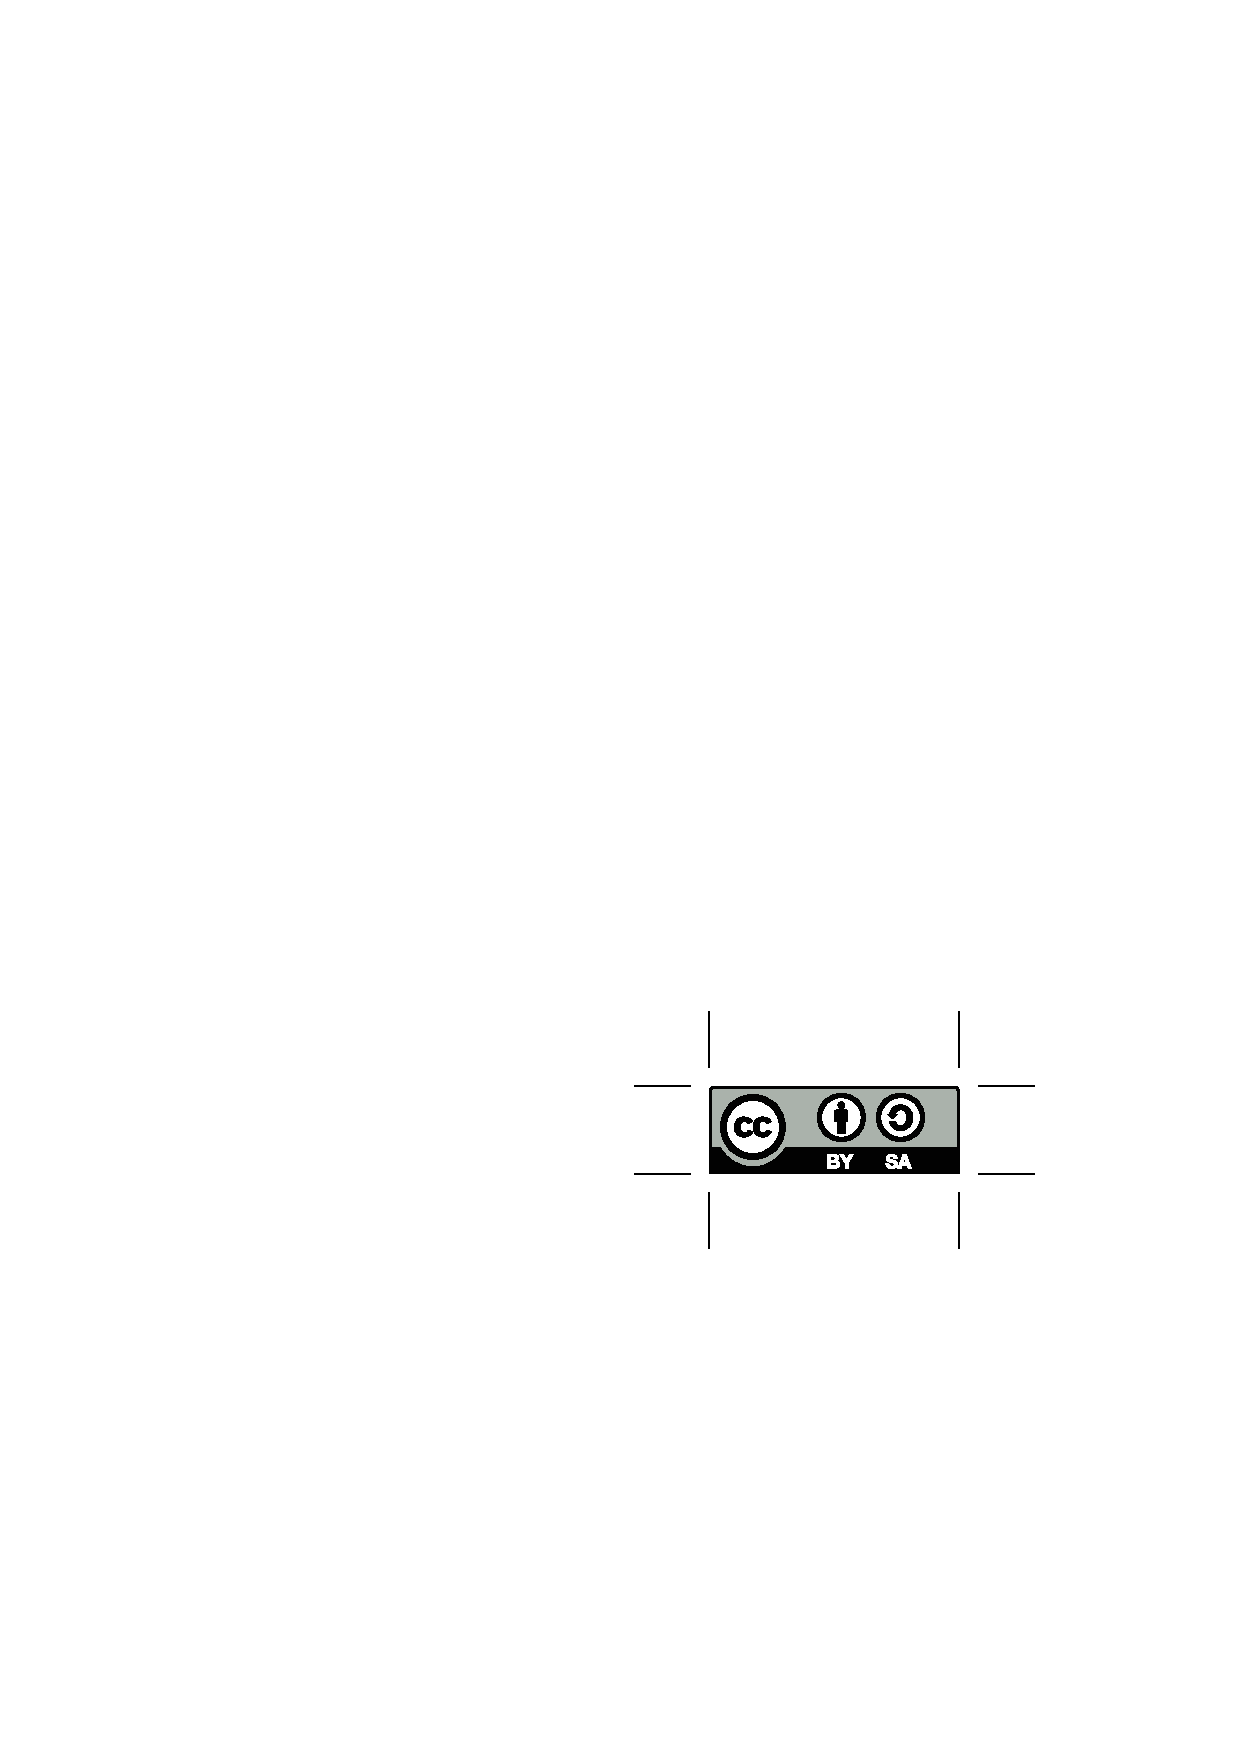
\includegraphics[scale=0.6]{img/by-sa}
	%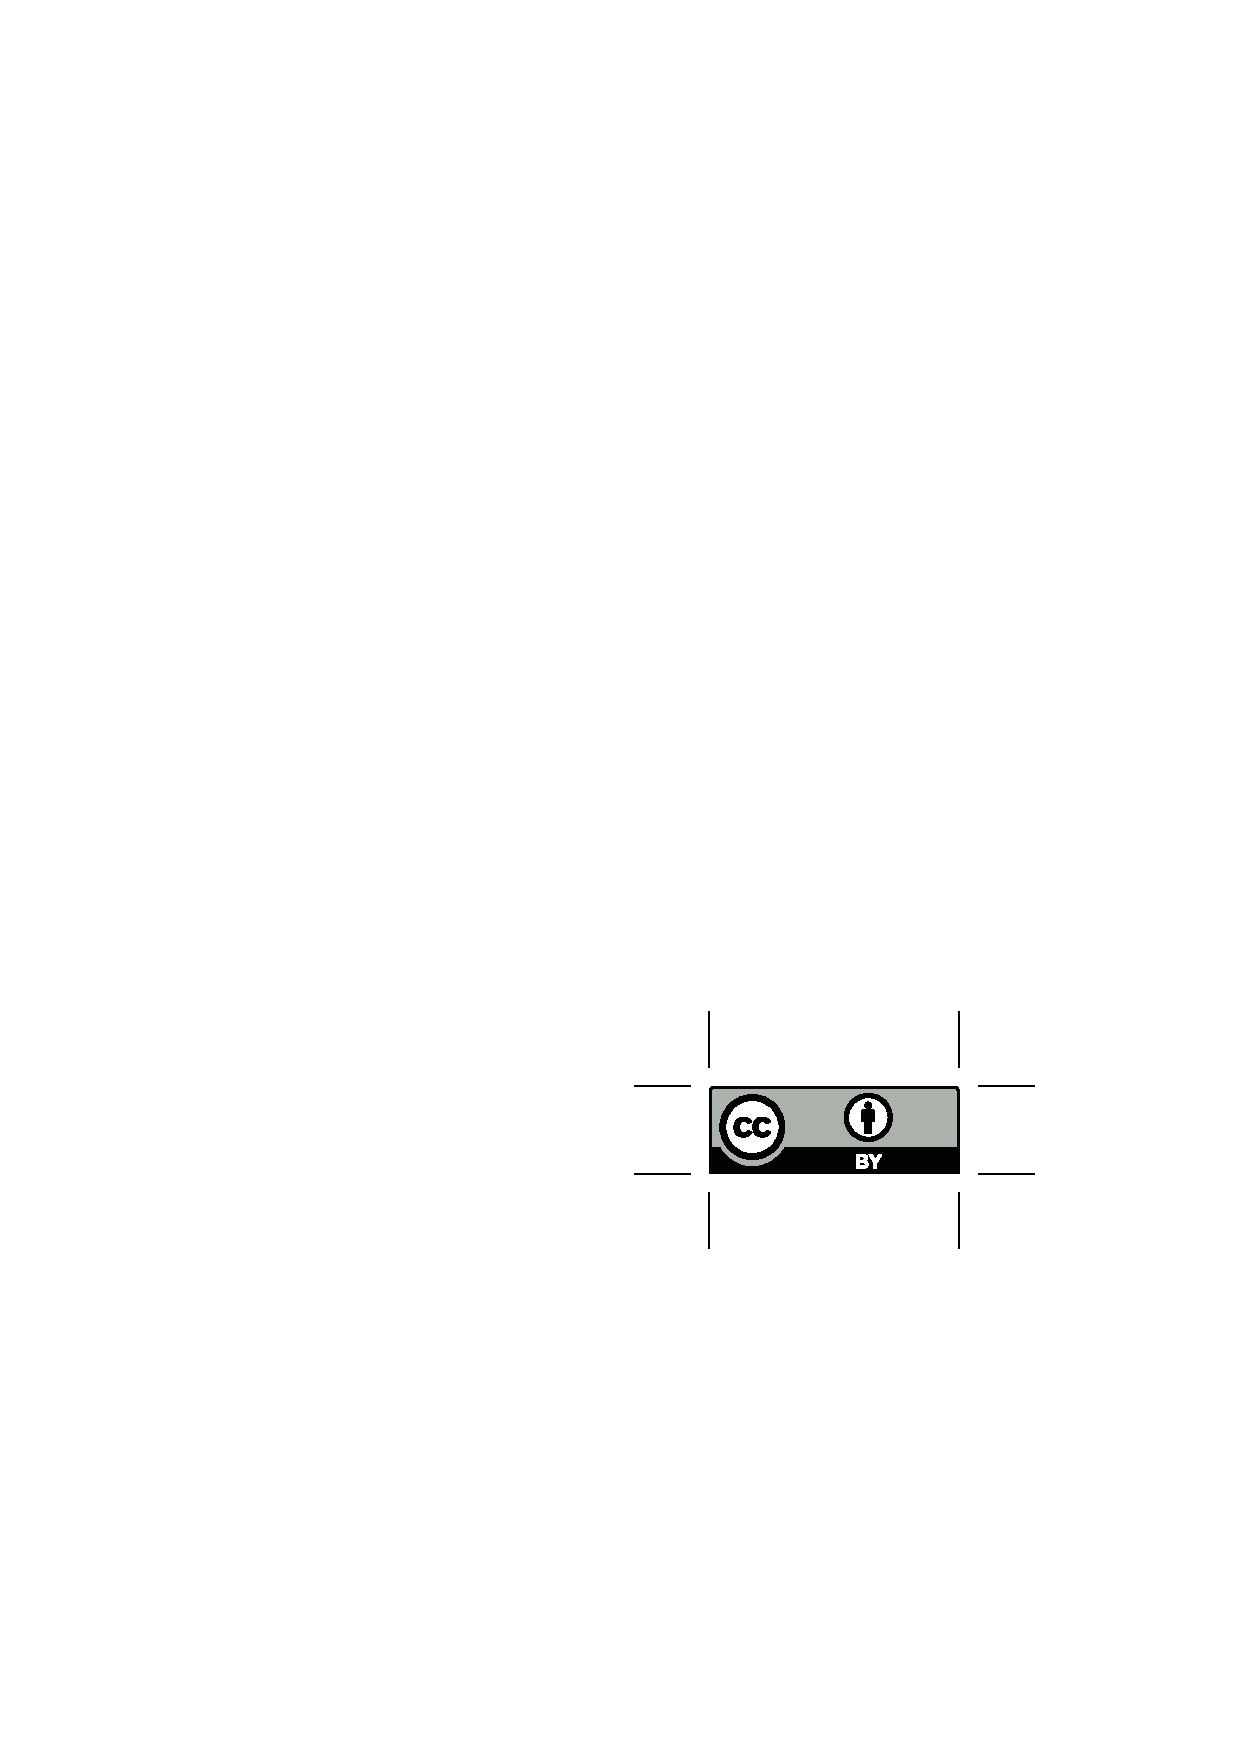
\includegraphics[scale=0.6]{img/by}

	%% Poner el año adecuado
	\noindent©2025 \theauthor  \\
	Algunos derechos reservados  \\
	Este documento se distribuye bajo la licencia \\
	``Atribución-CompartirIgual 4.0 Internacional'' de Creative Commons, \\
	disponible en \\
	\url{https://creativecommons.org/licenses/by-sa/4.0/deed.es}
\end{flushright}

%%%%%%%%%%%%%%%%%%%%%%%%%%%%%%%%%%%%%%%%%%%%%%%%%%%%%%%%%%%%%%%%%%%%%%%%%%%%%%%%
%%%% Dedicatoria

\chapter*{}
\pagenumbering{Roman} % para comenzar la numeracion de paginas en numeros romanos
\begin{flushright}
	\textit{Dedicado a \\
		todos aquellos que me animaron y apollaron \\
		incluso en mis momentos de debilidad}
\end{flushright}

%%%%%%%%%%%%%%%%%%%%%%%%%%%%%%%%%%%%%%%%%%%%%%%%%%%%%%%%%%%%%%%%%%%%%%%%%%%%%%%%
%%%% Agradecimientos

\chapter*{Agradecimientos}
%\addcontentsline{toc}{chapter}{Agradecimientos} % si queremos que aparezca en el índice
\markboth{AGRADECIMIENTOS}{AGRADECIMIENTOS} % encabezado 


%%%%%%%%%%%%%%%%%%%%%%%%%%%%%%%%%%%%%%%%%%%%%%%%%%%%%%%%%%%%%%%%%%%%%%%%%%%%%%%%
%%%% Resumen

\chapter*{Resumen}
%\addcontentsline{toc}{chapter}{Resumen} % si queremos que aparezca en el índice
\markboth{RESUMEN}{RESUMEN} % encabezado


%%%%%%%%%%%%%%%%%%%%%%%%%%%%%%%%%%%%%%%%%%%%%%%%%%%%%%%%%%%%%%%%%%%%%%%%%%%%%%%%
%%%% Resumen en inglés

\chapter*{Summary}
%\addcontentsline{toc}{chapter}{Summary} % si queremos que aparezca en el índice
\markboth{SUMMARY}{SUMMARY} % encabezado

%%%%%%%%%%%%%%%%%%%%%%%%%%%%%%%%%%%%%%%%%%%%%%%%%%%%%%%%%%%%%%%%%%%%%%%%%%%%%%%%
%%%%%%%%%%%%%%%%%%%%%%%%%%%%%%%%%%%%%%%%%%%%%%%%%%%%%%%%%%%%%%%%%%%%%%%%%%%%%%%%
% ÍNDICES %
%%%%%%%%%%%%%%%%%%%%%%%%%%%%%%%%%%%%%%%%%%%%%%%%%%%%%%%%%%%%%%%%%%%%%%%%%%%%%%%%

% Las buenas noticias es que los índices se generan automáticamente.
% Lo único que tienes que hacer es elegir cuáles quieren que se generen,
% y comentar/descomentar esa instrucción de LaTeX.

%%%% Índice de contenidos
\tableofcontents
%%%% Índice de figuras
\cleardoublepage
%\addcontentsline{toc}{chapter}{Lista de figuras} % para que aparezca en el indice de contenidos
\listoffigures % indice de figuras
%%%% Índice de tablas
%\cleardoublepage
%\addcontentsline{toc}{chapter}{Lista de tablas} % para que aparezca en el indice de contenidos
%\listoftables % indice de tablas


%%%%%%%%%%%%%%%%%%%%%%%%%%%%%%%%%%%%%%%%%%%%%%%%%%%%%%%%%%%%%%%%%%%%%%%%%%%%%%%%
%%%%%%%%%%%%%%%%%%%%%%%%%%%%%%%%%%%%%%%%%%%%%%%%%%%%%%%%%%%%%%%%%%%%%%%%%%%%%%%%
% INTRODUCCIÓN cpitulo 1%
%%%%%%%%%%%%%%%%%%%%%%%%%%%%%%%%%%%%%%%%%%%%%%%%%%%%%%%%%%%%%%%%%%%%%%%%%%%%%%%%

\cleardoublepage
\chapter{Introducción}
\label{sec:intro} % etiqueta para poder referenciar luego en el texto con ~\ref{sec:intro}
\pagenumbering{arabic} % para empezar la numeración de página con números




%%%%%%%%%%%%%%%%%%%%%%%%%%%%%%%%%%%%%%%%%%%%%%%%%%%%%%%%%%%%%%%%%%%%%%%%%%%%%%%%
%%%%%%%%%%%%%%%%%%%%%%%%%%%%%%%%%%%%%%%%%%%%%%%%%%%%%%%%%%%%%%%%%%%%%%%%%%%%%%%%
% Tecnologias usadas capitulo 2 %
%%%%%%%%%%%%%%%%%%%%%%%%%%%%%%%%%%%%%%%%%%%%%%%%%%%%%%%%%%%%%%%%%%%%%%%%%%%%%%%%

\cleardoublepage % empezamos en página impar
\chapter{Tecnologías utilizadas} % título del capítulo (se muestra)
\label{chap:objetivos} % identificador del capítulo (no se muestra, es para poder referenciarlo)
En esta sección se muestran las distintas tecnologías que han sido necesarias para el desarroyo de este proyecto tanto de forma directa como indirecta.
\section{Tecnologías principales} % título de sección (se muestra)
\label{sec:objetivo-general} % identificador de sección (no se muestra, es para poder referenciarla)

Aquí se nombran y explican aquellas tecnologías que han tenido una implicación directa con el proyecto y que han tenido un papel crucial e imprescindible con las cuales, sin ellas, no se habria popido llegar a los resultados obtenidos. 

\subsection{HTML5}
\label{subsec:HTML5}

HTML5 es la quinta iteración del lenguaje de HTML (\textit{marcado de hipertexto}), el cual es la estructura básica y principal de toda página web.
Desarrollado conjuntamente por W3C (\textit{World Wide Web Consortium}) y WHATWG (\textit{Web Hypertext Application Technology Working Group}).
HTML5 introduce mejoras sustanciales respecto a sus anteriores versiones, incluyendo nuevas etiquetas semánticas, soporte multimedia mejorado y compatibilidad
ampliada con diversos navegadores y dispositivos, dándole mayor flexibilidad y dinamismo a la creación de páginas web.

Una de sus nuevas introducciones clave es la introducción de etiquetas semánticas como: \texttt{<header>}, \texttt{<article>}, \texttt{<section>} y \texttt{<footer>},
que facilitan una estructuración clara y accesible del contenido web. Estas etiquetas no solo ayudan a mejorar la organización de la información, si no que también facilitan la búsqueda
de información por parte de los motores de búsqueda y facilitan la interpretación por parte de los desarrolladores.
Además, HTML5 incorpora nuevas interfaces de programación de aplicaciones (\textit{API}), destacándose las funcionalidades de almacenamiento local mediante
\texttt{localStorage} y \texttt{sessionStorage}, que permiten la gestión eficiente de datos directamente en el navegador, eliminando la necesidad de bases de datos externas. \cite{freeman2018head}

HTML5 también introduce mejoras significativas en la gestión de contenido multimedia, eliminando la necesidad de complementos externos. Para esto se implementaron
las etiquetas \texttt{<audio>} y \texttt{<video>} las cuales permiten la incorporación directa de archivos de sonido y video en las páginas web, permitiendo mayor dinamismo en el desarrollo.
Otro elemento que se añadió fue el elemento \texttt{<canvas>} el cual habilita la generación de gráficos y animaciones en tiempo real a través de JavaScript, permitiendo el desarrollo de aplicaciones interactivas y videojuegos en línea.

HTML5 se ha establecido firmemente como un estándar en el desarrollo de aplicaciones web progresivas (\textit{PWA}) y en entornos multiplataforma. Su integración con tecnologías como CSS3 y JavaScript
permite la creación de interfaces dinámicas y adaptativas, compatibles con una amplia gama de dispositivos, desde ordenadores hasta tabletas y teléfonos.

\subsection{JavaScript}
\label{subsec:JavaScript}
JavaScript es un lenguaje de programación ligero y multiplataforma utilizado principalmente para la creación de contenido dinámico e interactivo para páginas web.
Su felixibilidad permite desarrollar elementos para mejorar la interacción del usuario en páginas web tanto del lado del servidor como del lado del cliente. En 1997, JavaScript fue estandarizado
por \textit{ECMA} como ECMAScript y poco después como un éstandar \textit{ISO}.

JavaScript, creado por Brendan Eich de Netscape en 1995 bajo el nombre de \textit{Mocha}, posteriormente se renombró a LiveScript y finalmente a JavaScript.
En el año 2000, JavaScript se extendió al lado de los servidores con la introducción de tecnologías como \textit{Node.js}, y posteriormente su popularidad creció con la llegada de \textit{AJAX}. Y Con la llegada de ECMAScript 6 en 2015, se introdujeron características mas avanzadas y
actualizaciones anuales, haciendo que hoy en día sea uno de los lenguajes mas importantes en el desarrollo web.

JavaScript es un lenguaje de programación de alto nivel, lo que significa que su leguaje esta diseñado para ser lo mas 'humano' posible, permitiendo una rapida comprensión del codigo sin necesidad de un nivel alto de conocimientos.
Es un lenguaje basado en eventos ya sean entradas de ratón o entradas de teclado, permitiendo la creación de interfaces de usuario interactivas. JavaScript puede integrarse en un HTML dentro de la etiqueta \texttt{<script>} de forma directa, escribiendo el codigo.
También, se puede introducir codigos de JavaScript, los cuales estén en archivos distintos con la extensión correspondiente al lenguaje (.js), esto es posible vinculando dicho archivo en la cabecera del HTML.

\subsection{WebXR}
\label{subsec:WebXR}

WebXR \cite{onirix2024} es una tecnología desarrollada por W3C (\textit{World Wide Web Consortium}) que permite crear experiencias inmersivas desde el navegador. Esta tecnología combina la Realidad Aumentada (\textit{AR}) y la Realidad Virtual (\textit{VR}) con la accesibilidad de un navegador web.
Lo cual permite a los usuarios experimentar e interactuar con entornos tridimensionales a través de cualquier dispositivo con acceso a un navegador compatible.

A medida que la tecnología de WebXR ha ido evolucionando, se han desarrollado distintos tipos de experiencias para poder adaptarse a distintos contextos y necesidades. Hoy en día, se podria clasificar los distintos tipos en 3 categorias:
\begin{itemize}
	\item \textbf{WebXR AR:} Este tipo de WebXR combina el mundo virtual y el mundo real, permitiendo que distintos elementos del mundo virtual puedan superponerse en el entorno físico a través
	      de la cámara de un dispositivo compatible, pero sin que llegue a influir el mundo real en los elementos virtuales.
	\item \textbf{WebXR VR:} Este modo permite a los usuarios sumergirse en el entorno virtual creado, y con la ayuda de dispositivos suplementarios como auriculares, la experiencia es aún mayor. Esta tecnología permite a los usuarios
	      interactuar y experimentar en primera persona distintos entornos virtuales, desde juegos y entretenimiento, hasta simulaciones virtuales y visualizaciones en 3D.
	\item \textbf{WebXR MR(Mixed Reality):} Esta tecnología combina el mundo real y el virtual de forma mas profunda que la tecnología AR. Permite a los usuarios poder interactuar con elementos tantos virtuales como físicos y que estos puedan interactuar entre si. Este tipo de combinación proporciona un nivel mayor de interacción entre el usuario y
	      y su entorno, dando mayor numero de posibilidades para la creación de contenido.
\end{itemize}

Estos distintos tipos de WebXR ofrecen distintos tipos de experiencias dependiendo del entorno virtual que se quiera diseñar.

\subsection{WebLG}
\label{subsec:WebLG}
WebGl (\textit{Web graphics Library}), se trata de una tecnología de bajo nivel multiplataforma usada para la renderización de gráficos tanto tridimensionales como bidimensionales dentro de cualquier navegador que sea compatible.

WebGl fue lanzado en 2011 por el grupo Khronos. Esta tecnología se fundamenta en OpenGL ES, la cual es una variante simplificada de OpenGL, diseñada para dispositivos moviles. WebGL ha sufrido numerables actualizaciones, 
lo cual ha permitido una evolución continua que ha ido mejorando tanto su funcionalidad como compatibilidad tanto en navegadores de escritorio como en navegadores en dispositivos móviles. 

WebGL esta diseñado para trabajar directamente con la GPU (\textit{Graphic Processing Unit}) del dispositivo, lo cual permite un mayor aprovechamiento de la computación para poder generar gráficos detallados y de alta calidad. 
Además, la tecnología de WebGL esta diseñada para poder integrarse de manera fluida con otros estandares de desarrollo web como HTML, CSS o DOM. 

\subsection{Three.js}
\label{subsec:Three.js}

Three.js \cite{threejs_wikipedia} es una biblioteca de codigo abierto de JavaScript utilizada para la creación de gráficos 3D en los navegadores web. Three.js funciona sobre WebGL \cite{webgl_encodebiz}, la cual permite generar y visualizar animaciones y escenas 3D en el navegador sin necesidad de complementos. La tecnologia de WebGL tambiénpuede usarse junto con el elemento \texttt{<canva>} de HTML.

Esta biblioteca proporciona una API de alto nivel la cual permite al usuario la creación y manipulación de geometrías 3D como cubos, esfera o planos, así como la aplicación de texturas o la aplicación de tanto camaras como de efectos de iluminación en las escena, permitiendo que el desarrollo de dichas escenas sea mucho mas simplificado. 
También, Three.js permite la posibilidad de importar modelos 3D desde archivos distintos creados desde aplicaciones distintas.

La biblioteca de Three.js ofrece una alta variedad de herramientas que permiten la gestión y control de usuario, facilitando asi tanto la navegación como la interacción dentro de las escenas 3D. También, Three.js soporta animaciones suaves y dinámicas tanto para objetos en la escena como para camaras, lo cual permite la creación de efectos visuales mas dinámicos e impresionantes al igual que juegos interactivos. 


\subsection{A-frame}
\label{subsec: Aframe}

A-Frame \cite{aframe_docs} es un web framework diseñado para construir experiencias de realidad virtual. A-frame esta basado en HTML y en JavaScript, permitiendo realizar cualquier escena que uno pueda imaginar sin necesidad de conocimientos avanzados en gráficos 3D. 
Al estar basado en HTMl es posible realizar escenas simples directamente desde un archivo HTML simplemente importando la libreria de A-frame y añadiendo dentro de la etiqueta \texttt{<a-scene>} cualquier elemento que desee el usuario.  

Uno de los ejemplos más simples de A-frame es el siguiente:

\begin{lstlisting}[language=HTML, caption=Escena A-Frame básica, captionpos=b]
  <html>
    <head>
      <script src="https://aframe.io/releases/1.6.0/aframe.min.js"></script>
    </head>
    <body>
      <a-scene>
        <a-box position="-1 0.5 -3" rotation="0 45 0" color="#4CC3D9"></a-box>
        <a-sphere position="0 1.25 -5" radius="1.25" color="#EF2D5E"></a-sphere>
        <a-cylinder position="1 0.75 -3" radius="0.5" height="1.5" color="#FFC65D"></a-cylinder>
        <a-plane position="0 0 -4" rotation="-90 0 0" width="4" height="4" color="#7BC8A4"></a-plane>
        <a-sky color="#ECECEC"></a-sky>
      </a-scene>
    </body>
  </html>
\end{lstlisting}

Este código de HTML genera una de las escenas más básicas que se pueden hacer en A-frame. La cual consiste en un plano y, encima, una serie de figuras geométricas, como se aprecia en la figura \ref{fig:aframe-basic}.

\begin{figure}[H]  % requiere \usepackage{float}
  \centering
  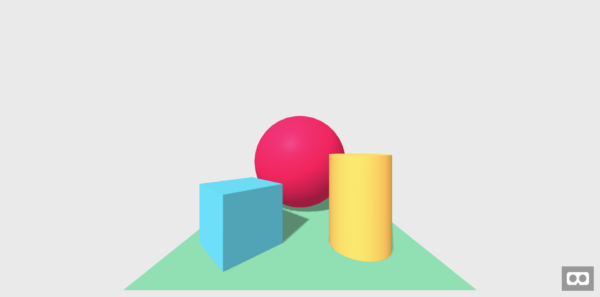
\includegraphics[width=0.7\textwidth]{img/aframe_hello_world.png}
  \caption{Escena básica de A-frame}
  \label{fig:aframe-basic}
\end{figure}

Una de las principales características de esta tecnología es su arquitectura basada en un modelo de entidad-componente (\textit{Entity Component System}), donde cada objeto dentro de la escena es una entidad que luego es integrada con Three.js para crear la escena.
Una entidad en A-frame es un objeto HTML que se crea añadiendo la etiqueta \texttt{<a-entity>} y el componente es la apariencia, comportamiento y funcionalidad que se le asigna mediante JavaScript. 

Para hacer uso de un componente se requiere de una serie de pasos previos. Si el componente es externo es necesario importarlo en la cabecera del HTML del mismo modo que se importa A-frame y posteriormente añadirlo a la entidad en la que uno desee usarlo. 
Por otra parte, si el  componente es de nuestra creación, primero hay que registrar y definir el componente. Esto se hace en un archivo externo de JavaScript mediante el método de \texttt{AFRAME.registerComponente}. A este método, del mimo modo que una función primero se le asigna un nombre, 
este sera el nombre del componente. Luego, este metodo consta de varias funciones internas las cuales se encargan de definir la apariencia y lógica de dicho componente. Alguna de estas funciones son la función \texttt{schema}, \texttt{init} o \texttt{tick}.
La función \texttt{schema}, define las propiedades principales del componente, estas se pueden modificar dependiendo de la lógica del componente desde el HTML a la hora de llamarlo. La función \texttt{init} se ejecuta una única vez al inicio cuando se inicializa el componente y la función \texttt{tick} se ejecuta a cada frame de la escena.
Una vez el componente esta registrado y programado importamos el archivo que contiene el componente al HTML y lo insertamos a la escena en la entidad u objeto que deseemos. 

Un ejemplo de la llamada de un componente dentro de un archivo de HTML se puede apreciar en \ref{lst:aframe-entity}
\begin{lstlisting}[language=HTML, caption=Ejemplo de entidad en A-frame, captionpos=b, label=lst:aframe-entity]
  <html>
    <head>
      <script src="https://aframe.io/releases/1.6.0/aframe.min.js"></script>
      <script src = "componente1.js"></script>
      <script src = "componente2.js"></script>
    </head>
    <body>
      <a-scene>
        <a-entity componente1></a-entity>
        <a-box componente2></a-box>
      </a-scene>
    </body>
  </html>
\end{lstlisting}

En este ejemplo primero se muestra como a una entidad vacia se le añade un compoennte llamado \texttt{componente1} y también se muestra como a una entidad de cubo se le añade el componente \texttt{componente2}.

\section{Tecnologias auxiliares}
\label{sec:tecnologias-auxiliares}
En esta sección se detallan y describen las distintas tecnologías que aunque no hayan influido de manera directa en los resultados del proyecto, han tenido un papel crucial para el desarroyo de este.


\subsection{Visual Studio Code}
\label{subsec: visualstudiocode}

Visual Studio Code (\textit{VS Code}) es un potente editor de código abierto el cual esta disponible para Windows, Linux, MacOS y versión web. VS Code es una de las plataformas de edición de codigo más utilizadas a nivel mundial 
por toda clase de desarrolladores de software debido a su versatilidad, flexibilidad y amplia gama de extensiones que facilitan la edición y depuración de código.

También, gracias a su pestaña de \textbf{Source Control}, permite ir guardando el código en GitHub para tener un control de las distintas versiones del código. 

Gracias a las numerosas extensiones que hay disponibles facilitan en gran medida la creación y depuración de código, permitiendo cosas como autocompletar palabras o expresiones o permitir compilar o depurar con algun lenguaje que VS Code no tenga por defecto.
Algunas de las extensiones utilizadas en este proyecto han sido: 
\begin{itemize}
  \item \textbf{A-frame completition}: Permite autocompletar rapidamente a la hora de escribir los distintos elementos o Snippets que posee A-frame
  \item \textbf{Error lens}: A la hora de depuración, permite visualizar dentro del código si hay algun error de sintaxis o lógica 
  \item \textbf{LaTeX Workshop}: Permite la escritura, compilación y previsualización de la memoria de este proyecto.
\end{itemize}

\subsection{Github}
\label{subsect:github}

GitHub es una plataforma basada en la nube que permite almacenar distintos repositorios y en cada repositorio codigo. Git fue creado en 2005 por Linus Torvalds como un sistema de control de versiones de código abierto.
Este sistema fue desarroyado con la intención de ayudar a los desarrolladores a tener en cualquier dispositivo con acceso a internet todo el historial de código que estan desarrollando. 

Esta tecnología es ampliamente utilizada a nivel mundial por desarrolladores de todo tipo debido a su capacidad de almacenar, soportar y gestionar proyectos de toda clase. Una de las funciones clave que presenta la plataforma, es la capacidad de crear ramificaciones (branches). Esta opcion permite a los desarroyadores poder crear copias del codigo del repositorio en el que 
estan trabajando para poder trabajar en paralelo y posteriormete poder integrar los cambios realizados en paralelo al codigo principal. Esta opcion también permite que mas de un desarrollador pueda trabajar en el mismo codigo, haciendo que cada uno trabaje en paralelo en ramas distintas. 

% \subsection{Meta Quest 3}
% \label{subsec:metaquest}

% Meta Quest se trata de un dispositivo inalámbrico diseñado para disfrutar de contenido de realidad virtual (VR). Dicho dispositivo esta compuesto por unas gafas, un micrófono y auriculares integrados en un unico dispositivo que el usuario pone en su cabeza y un par de mandos inalámbricos. 
% La primera version fue lanzada en 2020 con las Meta Quest 2 y 3 años mas tarde, en 2023 se lanzaron las Meta Quest 3. 


\subsection{LaTeX}
\label{subsec:latex}

LaTeX \cite{latexproject_about} es un software de uso libre de creación de documentación de alta calidad. Este sistema es altamente utilizado para la creación de documentación tecnica o cientifica de media o larga extensión, aunque gracias a su versatilidad se puede utilizar para cualquier tipo de documentación.

Entre las distintas caracteristicas de LaTeX cabe destacar su capacidad de manejar expresiones matematicas complejas, lo cual es una herramienta indispensable para cualquier documento cintifico. También gracias a su software motor TeX LaTeX es capaz de convertir los comandos de texto, utilizados para expresar los resultados tipográficos, en un archivo PDF profesional. 

Además de facilitar la creación de formulas matematicas complejas, LaTeX también ofrece otras facilidades avanzadas, como puede ser la creación de un índice del contenido, un índice de las figuras utilizadas, gestión de bibliografias o referencias simplificando la organización del documento y la citación de figuras o elementos externos en la bibliografia.
%%%%%%%%%%%%%%%%%%%%%%%%%%%%%%%%%%%%%%%%%%%%%%%%%%%%%%%%%%%%%%%%%%%%%%%%%%%%%%%%
%%%%%%%%%%%%%%%%%%%%%%%%%%%%%%%%%%%%%%%%%%%%%%%%%%%%%%%%%%%%%%%%%%%%%%%%%%%%%%%%
% {Desarrollo del proyecto copitulo 3 %
%%%%%%%%%%%%%%%%%%%%%%%%%%%%%%%%%%%%%%%%%%%%%%%%%%%%%%%%%%%%%%%%%%%%%%%%%%%%%%%%

\cleardoublepage
\chapter{Desarrollo del proyecto}
\label{chap:Desarrollo del proyecto}


%%%%%%%%%%%%%%%%%%%%%%%%%%%%%%%%%%%%%%%%%%%%%%%%%%%%%%%%%%%%%%%%%%%%%%%%%%%%%%%%
%%%%%%%%%%%%%%%%%%%%%%%%%%%%%%%%%%%%%%%%%%%%%%%%%%%%%%%%%%%%%%%%%%%%%%%%%%%%%%%%
% RESULTADOS capitulo 4%
%%%%%%%%%%%%%%%%%%%%%%%%%%%%%%%%%%%%%%%%%%%%%%%%%%%%%%%%%%%%%%%%%%%%%%%%%%%%%%%%

\cleardoublepage
\chapter{Resultados}
\label{chap:resultados}


%%%%%%%%%%%%%%%%%%%%%%%%%%%%%%%%%%%%%%%%%%%%%%%%%%%%%%%%%%%%%%%%%%%%%%%%%%%%%%%%
%%%%%%%%%%%%%%%%%%%%%%%%%%%%%%%%%%%%%%%%%%%%%%%%%%%%%%%%%%%%%%%%%%%%%%%%%%%%%%%%
% CONCLUSIONES capitulo 5%
%%%%%%%%%%%%%%%%%%%%%%%%%%%%%%%%%%%%%%%%%%%%%%%%%%%%%%%%%%%%%%%%%%%%%%%%%%%%%%%%

\cleardoublepage
\chapter{Conclusiones}
\label{chap:conclusiones}


\section{Aplicación de lo aprendido}
\label{sec:aplicacion}



\section{Lecciones aprendidas}
\label{sec:lecciones_aprendidas}


\section{Trabajos futuros}
\label{sec:trabajos_futuros}

%%%%%%%%%%%%%%%%%%%%%%%%%%%%%%%%%%%%%%%%%%%%%%%%%%%%%%%%%%%%%%%%%%%%%%%%%%%%%%%%
%%%%%%%%%%%%%%%%%%%%%%%%%%%%%%%%%%%%%%%%%%%%%%%%%%%%%%%%%%%%%%%%%%%%%%%%%%%%%%%%
% BIBLIOGRAFIA %
%%%%%%%%%%%%%%%%%%%%%%%%%%%%%%%%%%%%%%%%%%%%%%%%%%%%%%%%%%%%%%%%%%%%%%%%%%%%%%%%

\cleardoublepage

% Las siguientes dos instrucciones es todo lo que necesitas
% para incluir las citas en la memoria
\bibliographystyle{abbrv}
\bibliography{memoria}  % memoria.bib es el nombre del fichero que contiene
% las referencias bibliográficas. Abre ese fichero y mira el formato que tiene,
% que se conoce como BibTeX. Hay muchos sitios que exportan referencias en
% formato BibTeX. Prueba a buscar en http://scholar.google.com por referencias
% y verás que lo puedes hacer de manera sencilla.
% Más información: 
% http://texblog.org/2014/04/22/using-google-scholar-to-download-bibtex-citations/

\end{document}
